\section{Literature Review}
% \addcontentsline{toc}{section}{Literature Review}
\fancyhead[R]{Literature Review}

\subsection{Enzymatic Mechanisms Involved in Pesticide Breakdown}
\label{sec:Enzymatic Mechanisms Involved in Pesticide Breakdown}

The degradation of pesticides in the environment is a complex process and occurs by various mechanisms, but mainly through microbial enzymatic activities. The enzymes catalyze reactions in which toxic pesticide compounds are transformed into less harmful compounds facilitating their removal from the environment. In this part, the most critical enzymatic mechanisms applied in pesticide degradation are hydrolytic, oxidative, and reductive enzymes.

Microbial enzymes play critical roles in the biodegradation of soil contaminants, one of which is pesticides. They can further be classified based on the reactions they catalyze:

\textbf{Hydrolytic Enzymes:} Hydrolytic enzymes are divided into two groups, esterases and amidases, which hydrolyze ester and amide bonds in pesticide molecules. Their hydrolysis changes them into compounds of much smaller size and more water solubility, which can easily be eliminated through further degradation. For example, microbial esterases act upon organophosphate insecticides in their rapid degradation to hydrolyze them.

\textbf{Oxidative Enzymes:} This group of oxidative enzymes includes cytochrome P450 monooxygenases, which introduce oxygen atoms into molecules of pesticides, thus increasing their solubility and reactivity. Commonly, this oxidation makes the pesticides less hazardous, or other enzymes can further degrade the intermediates formed. In particular, the cytochrome P450 enzymes are very versatile, able to metabolize a vast range of xenobiotics, including pesticides.

For example, reductive enzymes catalyze the reduction of pesticides, in most cases by donating electrons and hydrogen atoms on the molecules. Such a reduction may well break complex structures that facilitate the conversion of pesticides into simpler forms that are much less toxic. For instance, reductive dehalogenases are believed to be important in breaking down halogenated organic compounds.

Degradation of pesticides in contaminated soils by the use of microbial enzymes in bioremediation strategies significantly improves the degradation of the pesticides. The approach is based on the natural capability of microbes to detoxify pollutants via enzymatic reactions. A review found that the efficiency of microbial enzymes in the degradation of pesticides contaminated in soil was well established. \autocite{singhMicrobialDegradationOrganophosphorus2006} Further study focused on the developments and applications of microbial enzymes for enhancing the process of biodegradation. This review will focus on the critical role of enzymes in pesticide-degradation pathways and discuss the potential for engineered enzymes to increase bioremediation efficiency. \autocite{chiaFunctionMicrobialEnzymes2024}

Understanding the enzymatic mechanisms is crucial for predicting the enzymatic classes responsible for pesticide degradation. By analyzing the interactions between enzymes and pesticides, it is possible to identify the specific enzyme classes involved in the degradation process. This knowledge can inform the development of more accurate predictive models for pesticide degradation, enabling better risk assessments and environmental management strategies.

\subsection{Deep Learning Techniques in Environmental Science}
\label{sec:Deep Learning Techniques in Environmental Science}

Deep Learning has been an essential tool in environmental science, enabling advanced prediction and understanding complex biochemical processes. There are several Deep Learning architectures such as the protein-transformer ESM model, which has made a significant impact on predicting biological properties from sequence data. \autocite{rivesBiologicalStructureFunction2021}

In the context of pesticide degradation and enzyme classification, such models can analyze large quantities of available biochemical data to make predictions about enzyme interactions and functions. Several deep learning architectures have been applied in enzyme classification and prediction tasks, from which valuable insights into the mechanism of pesticide degradation can be obtained.

For instance, the DEEPre model applies deep learning to predict enzyme commission (EC) numbers based on raw sequence data. Such models apply convolutional and sequential feature extraction techniques, leading to significant improvements in prediction accuracy over methods in current use. In this respect, such models may play a key role in predicting the pesticide biodegradation pathways and help to make environmental risk assessment more precise and fast. \autocite{liDEEPreSequencebasedEnzyme2017}

The DeEPn model is one of the examples when EC classification has been done using a deep neural network for enzymes being classified into their functional classes, including all seven EC classes. This model has shown high precision and accuracy and, hence could become an essential tool for environmental scientists interested in understanding and predicting enzyme-mediated degradation processes. The proper classification of enzymes through DeEPn can help predict potential candidates for bioremediation, among other applications related to the environment. \autocite{DeEPnDeepNeural}

Despite the advances made by these models, there is still a need for new approaches to further improve the accuracy of sequence based predictions. Traditional models often rely on pre-defined features and limited datasets, which can restrict their performance and generalizability. In addition to this, the existing methods only focus on the prediction to the 3rd level of the EC classification, which may not provide sufficient detail for predicting pesticide degradations. For example the accuracy of EnzymeNet, a residual neural network model, across all the sub-subclasses is 0.398. In addition to that there is no score for the 4th level. The following picture shows the macro F1 score for diffrent models and EnzymeNet, which is the best one, but still not good enough. Therefore, there is a need for more advanced deep learning models that can predict enzyme classes with higher accuracy and resolution, enabling more precise predictions of pesticide degradation pathways. \autocite{watanabeEnzymeNetResidualNeural2023}
\begin{figure}[hbt]
    \centering
    \begin{minipage}[t]{.8\textwidth}
    \caption{Macro F1 score for different models and EnzymeNet}
    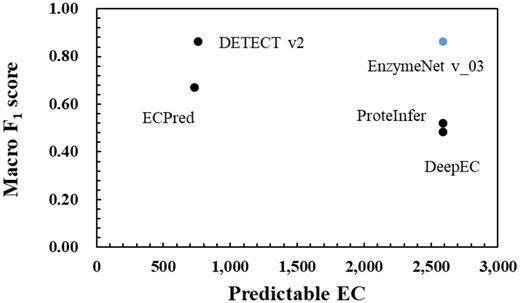
\includegraphics[width=1\textwidth]{img/performance_existing_methods.png}
    \source{Watanabe et al. (2023)}
    \label{fig:EnzymeNet}
    \end{minipage}
\end{figure}

By contrast, the proposed approach leverages the deep learning tool p2rank to analyze the interactive parts of enzymes, focusing on the ligand-binding sites and the specific amino acids involved.  This method can potentially provide a more detailed and accurate prediction of enzyme classes responsible for pesticide degradation, enhancing our understanding of the biodegradation pathways and mechanisms involved. \autocite{krivakP2RankMachineLearning2018}